\chapter{Optimal Transport Theory}

To introduce the optimal transport problem please imagine we are asked by a consortium of factories to design a plan for distributing their products among its many customers in such a way that the transportation costs are minimal. \\


We can start the approach of this problem considering the customers as members of the set $X$ and the factories as members of a set $Y$. We want to know which factory $y\in Y$ is going to supply a customer $x\in X$, i.e. we represent such assignation of a factory to a customer as map $y=T(x)\in Y$. Therefore, we can estimate the transportation cost $c(x, T(x))$ of supplying a customer $x$ with a factory $y=T(x)$. 

We see that our problem is reduced to find an assigning map from the set of customers to the set of factories in such a way that the total cost $C(X, Y)=\sum_{x\in X} c(x, T(x))$ is minimal.  
\\
\begin{figure}[H]
	\centering
	\caption{Illustration of the problem of Factories supplying customers.}
	\begin{subfigure}[t]{0.4\textwidth}
		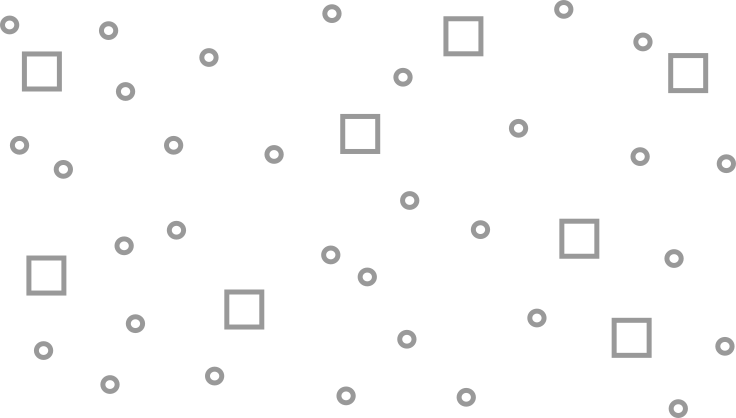
\includegraphics[width=\textwidth]{Factories-Customers.png}
		\caption{Factories represented by squares. customers represented by circles.}
	\end{subfigure}
	\hfil
	\begin{subfigure}[t]{0.4\textwidth}
		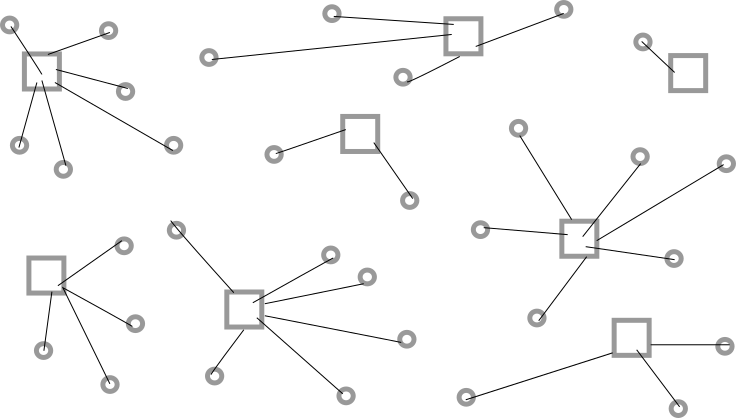
\includegraphics[width=\textwidth]{Factories-Customers-Assignation.png}
		\caption{Factories represented by squares. customers represented by circles. Assignation of a factory to a customer represented by a line.}
	\end{subfigure}	
\end{figure}

Gaspard Monge was a French mathematician who introduced for the very first time the optimal transport problem as \textit{d\'eblais et remblais} in 1781. Monge was interested in finding a map that distributes an amount of sand or soil extracted from the earth or a mine distributed according to a density $f$, onto a new construction whose density of mass is characterized by a density $g$, in such a way the average displacement is minimal. We see that Monge presented a more continuous flavor of the problem.

We remark that we are not interested in the quantity of mass we are transporting. This information it is not relevant for the problem or has no sense its consideration (for example the factories-customer problem). We are interested in finding a way to assign or distribute elements among two sets. We are interested in applications concerning the transportation of a finite amount of mass. Therefore, it is reasonable to state our problem in terms of probability measures.  

Formally, given two densities of mass $f$ and $g$, Monge was interested in finding a map $T:\Real^3\rightarrow\Real^3$ pushing the one onto the other,

\begin{equation*}
	\int_A g(y) \dy = \int_{T^{-1}(A)} f(x) \dx  \label{eq: Integral-Borel-MP}
\end{equation*}
For any Borel subset $A\subset\Real^3$. And the transport also should minimize the quantity, 
\begin{equation*}
	\int_{\Real^3} \abs{x-T(x)} f(x)\dx
\end{equation*}

Therefore, we need to search for the optimum in the set of measurables maps $T:X \rightarrow Y$ such that the condition \eqref{eq: Integral-Borel-MP} is translated to,

\begin{equation}
	(T_\#\mu)(A)=\mu(T^{-1}(A))
\end{equation}
for every measurable set $A$. In other words, we need $T_\# \mu = \nu$.  Notice that given the context for which the problem was formulated, originally it was binded to $\Real^3$ or $\Real^2$ but we can consider the general case in $\Real^d$. In the Euclidean frameworks if we assume $f$, $g$ and $T$ regular enough and $T$ also injective, this equality implies,
\begin{equation}
	g(T(x))\det\parentheses{\D T(x)}=f(x) \label{eq: PDE Monge condition.}
\end{equation} 
\begin{figure}[H]
	\centering
	\caption{Monge problem. Finding a map.}
	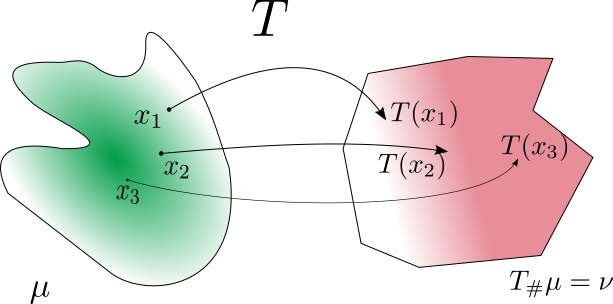
\includegraphics[width=0.4\textwidth]{Monge-Problem-densities.png}
\end{figure}

The equation \eqref{eq: PDE Monge condition.} is nonlinear in $T$ making difficult the analysis of the Monge's Problem. Moreover, the constrain makes this problem hard to handle since it is not close even under weak convergence. 


To appreciate this fact, consider $\mu = \Lebesgue^1\measurerestr[0,1]$ and the hat functions $h_k$ defined as follow,

\begin{equation*}
	h_k(x)=\begin{cases}
		2kx & x\in\brackets{0, \frac{1}{2k}}\\
		2-2kx & x\in \left(\frac{1}{2k}, \frac{1}{k}\right] \\
		0 & \otherwise
	\end{cases}
\end{equation*}
Then take the sequence $f_n:[0,1]\rightarrow [0,1]$,
\begin{equation}
	f_n(x)=\sum_{i=0}^{n-1}h_n\parentheses{x-\frac{i}{n}}
\end{equation}


We see that the sequence satisfies $\Tmeasure{\mu}{f_{n}}=\mu$. It is easy to check that $\mu\parentheses{f_n^{-1}\left(A\right)}=\Lebesgue^1\parentheses{A}$ for every open set $A\in [0,1]$. In the other hand, the sequence converges weakly to $f_n\weakconvergence f=\frac{1}{2}$, which obviously makes $\Tmeasure{\mu}{f}\neq\Lebesgue^1\measurerestr [0,1]$. 


\begin{problem} Given two probability measures $\mu \in \PlanSp\parentheses{X}$ and $\nu \in \PlanSp\parentheses{Y}$ and a cost function $c: X \times Y \rightarrow \braces{0, +\infty}$, the Monge's problem consists in finding a map $T:X\rightarrow Y$
	
\begin{equation}
\inf\braces{\Monge:=\int_X c(x, T(x)) \diff \mu(x): \ \ \Tmeasure{\mu}{T}=\nu }\label{eq: Monge's Problem.}\tag{MP}
\end{equation}
\end{problem}

Monge analyzed geometric properties of the solution to this problem. Although, the question of the existence of a optimal map stayed open until a Russian mathematician named Leonid Vitaliyevich Kantorovich introduced in the paper \cite{Kantorovich1942} a suitable framework to study its optimality conditions and prove existence of a minimizer. 

Formulating our factories-customer problem through finding an assignation map, we are excluding the situations in which one customer can be supplied by two or more factories, or for Monge's problem we are ignoring the possibility of splitting a unit of mass into small pieces that can be assigned simultaneously to different places. 

The idea behind Kantorovich's formulation is to consider instead of transportation maps from one space to another, transportation plans, that is joint probability measures with their marginals given by the initial and final configurations.

Instead of assigning an element of $Y$ to each element of the set $X$, we can see the problem from a different perspective and assign a weight to the importance of the point $\left(x, y\right)\in X\times Y$. In a better manner we would like to know how much of our total material is distributed in a way $(x, y)$ in such a way to be consistent with information we have the initial and final material configuration. We call this way to design the transportation strategy a transport plan. In terms of probability, we are constructing a joint probability measure for $X\times Y$ with marginals given by the measures $\mu \in \PlanSp(X)$ and $\nu \in \PlanSp(Y)$.

Please note that in contrast to a map, we can always assign to a point $x\in Y$ as many points in $Y$ as we want, just considering the constraints that we are not creating or destroying mass. 


We introduce the following notation. 

\begin{definition}[Coupling]
Let $\mu$ and $\nu$ be probability measures of a probability space $\parentheses{X, \mathcal{A}_X}$ and $\parentheses{Y, \mathcal{A}_Y}$. Finding a coupling between $\mu$ and $\nu$ means to construct a measure $\gamma$ on the space $X\times Y$ (precisely on the product $\sigma$-algebra $\mathcal{A}_X\otimes\mathcal{A}_Y$) such that $\mu$ and $\nu$ are admitted as marginals on $X$ and $Y$ respectively. That is the measure of the projections $\pi_x$ and $\pi_y$
\end{definition}
 
 Let $(X, \mu)$ and $(Y, \nu)$ be two probability spaces. Coupling $\mu$ and $\nu$ means constructing two random variables $\X$ and $\Y$ on some probability space $(\Omega, \mathcal{P})$ such that $\law(\X)=\mu$, $\law(\Y)=\nu$. The couple $(\X,\Y)$ is called a coupling of $(\mu, \nu)$.  
 
\begin{definition}[Deterministic Coupling]
A coupling $(\X,\Y)$ is said to be deterministic if there exists a measurable function $T: X \rightarrow Y$ such that $\Y = T(\X)$.
\end{definition}

The increasing rearrangement on $\Real$ is an example of a coupling between two probability measures over one dimensional euclidean space. Let $\mu$, $\nu$ be two probability measures on $\Real$. Define their cumulative distribution functions by,
\begin{equation*}
	F(x)=\int_{-\infty}^{x}\dmu, \qquad G(y)=\int_{-\infty}^{y}\dnu	
\end{equation*}
Cumulative distributions not always are invertible, since they are not always strictly increasing. Although we can define their pseudo-inverses as follow,
\begin{align}
	F^{-1}(t)=\inf\braces{x\in \Real; F(x)>t}; \label{eq: Increasing rearregement F}\\
	G^{-1}(t)=\inf\braces{y\in \Real; G(y)>t}; \label{eq: Increasing rearregement G}
\end{align}
and we set the map $T$ as,
\begin{equation}
	T=G^{-1}\circ F \label{eq: Increasing rearregement map.}
\end{equation}
We see if $\mu$ is atomless then $\Tmeasure{\mu}{T}=\nu$.

The above coupling is useful to construct the \textit{Knothe-Rosenblatt coupling} between two Stochastic variables $\Real^n$ is another interesting coupling. Let $\mu$ and $\nu$ be two probability measures on $\Real^n$, such that $\mu$ is absolutely continuous with respect to Lebesgue measure.  is constructed in the following way:

\begin{enumerate}
	\item Take the marginal of the first projection on the first variable; this gives probability measures $\mu_1\parentheses{\dx_1}$, $\nu_1\parentheses{\dy_1}$ on $\Real$, with $\mu_1$ being atomless. Then define $y_1=T_1(x_1)$ by the formula \eqref{eq: Increasing rearregement map.} with $F$ and $G$ considered as they are in \eqref{eq: Increasing rearregement F} and \eqref{eq: Increasing rearregement G} respectively.
	
	\item Now take the marginal on the first two variables and disintegrate it with respect to the first variable. This gives probability measures $\mu_2\parentheses{\dx_1\dx_2}=\mu(\dx_1)\mu_2(\dx_2 | \dx_1)$, $\nu_2 (\dy_1\dy_2)=\nu_1(\dy_1)\nu_2(\dy_2)$. Then, for each given $y_1\in \Real$, set $y_1=T_1(x_1)$, and then define $y_2=T_2(x_2; x_1)$ under the increasing rearrangement formula.  
\end{enumerate} 


\begin{lemma}[Gluing lemma] Let $(\X_i , \mu_i)$, $i = 1, 2, 3$,  be Polish probability spaces. If $(X_1 , X_2)$ is a coupling of $(\mu_1, \mu_2 )$ and $(\Y_2 , Y_3)$ is a coupling of $(\mu_2, \mu_3)$, then it is possible to construct a triple of random variables $(Z_1 , Z_2, Z_3)$ such that $(Z_1, Z_2)$ has the same law as $(X_1 , X_2)$ and $(Z_2, Z_3)$ has the same law as $(Y_2 , Y_3)$.
\end{lemma}

Notice that this way to see the problem is more general, since we can always create a transportation plan given a transportation map, i.e. 

\begin{equation*}
\Tmeasure{\mu}{(\id, T)}=\gamma \in \PlanSp(X\times Y)
\end{equation*}. 

If $T$ is a transportation map it is easy to check that indeed $\Tmeasure{\gamma}{\pi_x}=\mu$ and $\Tmeasure{\gamma}{\pi_y}=\nu$. The beauty of Kantorovich's formulation lies on the fact that it is always possible to find a transport. Moreover, the space of transport plans is compact.


\begin{problem}Given $\mu \in \PlanSp\parentheses{X}$, $\nu \in \PlanSp\parentheses{Y}$, and $c: X\times Y \rightarrow \brackets{0, +\infty}$, we consider the problem
	\begin{equation}
		\inf\braces{\Kantorovich := \int_{X\times Y} c \diff\gamma : \gamma \in \TransPlansSet{\mu}{\nu}}\label{eq: Kantorovich's Problem.}\tag{KP}
	\end{equation}
where $\TransPlansSet{\mu}{\nu}$ is the set of \textit{transport plans}.
\end{problem}




\section{Kantorovich formulation as relaxation}

\begin{theorem}
	Let $X$ and $Y$ be compact metric spaces, $\mu \in \PlanSp(X)$, $\nu \in  \PlanSp$ and
	$c:X\times Y \rightarrow \Real$  a continuous function. Then  \eqref{eq: Kantorovich's Problem.} admits a solution.
\end{theorem} 

\section{Cyclical Monotonicity.}

Consider a similar situation to the factories-customers example, but the consortium has already a fixed distribution plan. They know that transportation costs are high and they want to make them cheaper. 

\begin{definition}[c-transform]
	Let $X$ and $Y$ be sets, and $c:X\times Y \rightarrow (-\infty, \infty]$. A function $\psi: X\rightarrow \Realex$ is said to be c-convex if it is not identically to $+\infty$ and there exists $\psi^c: Y \rightarrow \Realex$
	
	\begin{equation}
		\psi^c(y)= \inf_{x\in X} c(x,y)-\psi(x).
	\end{equation}
\end{definition}

\begin{definition}
	Let $X , Y$ be arbitrary sets, and $c:X\times Y \rightarrow (-\infty, \infty]$ be a cost function. A subset $\Gamma \subset X \times Y$ is said to be c-cyclically monotone if, for any $N\in\Naturals$, and any family of points $(x_1, y_1), (x_2, y_2), \dots (x_N, y_N)$ of $\Gamma$, the inequality
	\begin{equation*}
		\sum_{i=1}^{N} c(x_i, y_i) \leq \sum_{i=1}^{N} c(x_i, y_{i+1}) 
	\end{equation*} 
	considering $N+1=1$. 
\end{definition}
Since any permutation $\sigma$ over the set $\braces{1, \dots, N}$ can be written as a product of disjoint cycles, we have that this property satisfies,
\begin{equation}
		\sum_{i=1}^{N} c(x_i, y_i) \leq \sum_{i=1}^{N} c(x_i, y_{\sigma(i)}) 
\end{equation}
\begin{definition}[Support of transport plan.]
	Given a separable metric space $X$, the support of a measure $\gamma$ is defined as the smallest closed set on which $\gamma$ is concentrated,
	\begin{equation}
	\spt(\gamma)\ :=\underset{\small{\begin{array}{c}
		\gamma(X\backslash A)=0\\ A=\bar{A}  \end{array}}}{\bigcap A} 		
	\end{equation} 
\end{definition}
We can fix a point $(x_0, y_0) \in \spt(\gamma)$, then 
\begin{theorem}
	
\end{theorem}

\section{Properties of Optimal plans.}
\section{Wasserstein Spaces. $\WassersteinSp{p}$}